\iffalse
\let\negmedspace\undefined
\let\negthickspace\undefined
\documentclass[journal,12pt,twocolumn]{IEEEtran}
\usepackage{cite}
\usepackage{amsmath,amssymb,amsfonts}
\usepackage{graphicx}
\usepackage{textcomp}
\usepackage{xcolor}
\usepackage{txfonts}
\usepackage{listings}
\usepackage{enumitem}
\usepackage{mathtools}
\usepackage{gensymb}
\usepackage{comment}
\usepackage[breaklinks=true]{hyperref}
\usepackage{tkz-euclide} 
\usepackage{listings}
\usepackage{gvv}                                        
\def\inputGnumericTable{}                                 
\usepackage[latin1]{inputenc}                                
\usepackage{color}                                            
\usepackage{array}                                            
\usepackage{longtable}                                       
\usepackage{calc}                                             
\usepackage{multirow}                                         
\usepackage{hhline}                                           
\usepackage{ifthen}                                           
\usepackage{lscape}
\usepackage[export]{adjustbox}

\newtheorem{theorem}{Theorem}[section]
\newtheorem{problem}{Problem}
\newtheorem{proposition}{Proposition}[section]
\newtheorem{lemma}{Lemma}[section]
\newtheorem{corollary}[theorem]{Corollary}
\newtheorem{example}{Example}[section]
\newtheorem{definition}[problem]{Definition}
\newcommand{\BEQA}{\begin{eqnarray}}
\newcommand{\EEQA}{\end{eqnarray}}
\newcommand{\define}{\stackrel{\triangle}{=}}
\newtheorem{rem}{Remark}

\begin{document}
\parindent 0px
\bibliographystyle{IEEEtran}

\vspace{3cm}

\title{}
\author{EE23BTECH11042 -  Khusinadha Naik$^{*}$
}
\maketitle
\newpage
\bigskip

% \renewcommand{\thefigure}{\theenumi}
% \renewcommand{\thetable}{\theenumi}


\section*{Exercise 5.2}

\noindent \textbf{18} \hspace{2pt}The sum of the 4th and 8th terms of an AP is 24 and the sum of the 6th and 10th terms is 44. Find the first three terms of the AP.\\
\noindent \textbf{Ans.}\\
\fi

\begin{table}[h]
\centering
\begin{tabular}{|c|c|c|}
        \hline
        \textbf{Parameter} & \textbf{Value} & \textbf{Description} \\
        \hline
        $x\brak{0}$ & ? & First term of AP \\
	\hline
	$d$ & ? & Common difference \\
        \hline
        $x\brak{3} + x\brak{7}$ & 24 & Sum of 4th , 8th term \\
        \hline
	$x\brak{5} + x\brak{9}$ & 44 & Sum of 6th , 10th term \\
	\hline
        $x(n)$ & $\brak{x\brak{0} + nd}u\brak{n}$ & General term \\
        \hline
\end{tabular}
\caption{Input parameters table}
\label{tab:10.5.2.18.1}



\end{table}

\noindent From \tabref{tab:10.5.2.18.1}

\begin{align}
x\brak{0}+3d + x\brak{0}+7d &= 24 \label{eq:10.5.2.18.1}\\
x\brak{0}+5d + x\brak{0}+9d &= 44 \label{eq:10.5.2.18.2}
\end{align}

\noindent Subtracting \eqref{eq:10.5.2.18.1} from \eqref{eq:10.5.2.18.2}

\begin{align}
4d &= 20 \\
\implies d &= 5  \label{eq:10.5.2.18.4}
\end{align}

\noindent Putting \eqref{eq:10.5.2.18.4} in \eqref{eq:10.5.2.18.1}

\begin{align}
2x\brak{0} + 10d &= 24 \\
2x\brak{0} + 10\brak{5} &= 24 \\
\implies x\brak{0} &= -13
\end{align}

Now , general term becomes
\begin{align}
x\brak{n} &= \brak{-13 + 5n}u\brak{n}
\end{align}

Taking Z-transform of $x\brak{n}$
\begin{align}
X\brak{z} = & \frac{-13}{1 - z^{-1}} + \frac{ 5z^{-1}}{\brak{1 - z^{-1}}^2}\\
X\brak{z}\implies & \frac{18z^{-1} - 13}{z^{-2} - 2z^{-1} + 1} \quad \text{, ROC: } |z| > 1 
\end{align}

\pagebreak

Plotting $x\brak{n}$ v $n$ :
\begin{figure}[h]
    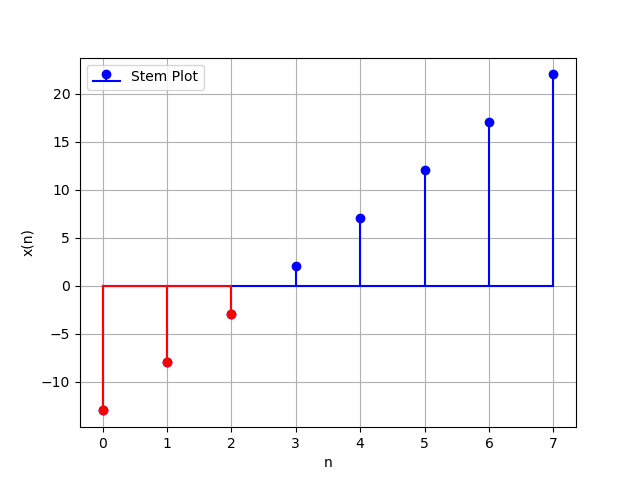
\includegraphics[width=0.5\textwidth]{ncert-maths/10/5/2/18/figs/fig1.png}
    \caption{Given AP}
    \label{fig:10.5.2.18.1}
\end{figure}

From \figref{fig:10.5.2.18.1} first three terms will be
\begin{align}
\{x\brak{0},x\brak{1},x\brak{2}\} &= \{-13 , -8 , -3\}
\end{align}















%\end{document}
